\documentclass{hsflensburg}
\title{Bewegungserkennung auf mobilen Geräten mit Verwendung von GANs für eine
automatische Datensatzgenerierung}
\subtitle{Master-Thesis}

\author{
  \name{Florian Hansen}\\
  \institution{Hochschule Flensburg}
}

\usepackage[ngerman]{babel}
\usepackage{csquotes}
\usepackage{biblatex}
\usepackage{amsmath}
\usepackage{amssymb}
\usepackage{mathtools}
\usepackage[ngerman,linesnumbered,algoruled,boxed,lined]{algorithm2e}
\addbibresource{bibliography.bib}

\newtheorem{definition}{Definition}

\setcapindent{0pt}

\begin{document}
  \maketitle
  \newpage \ \newpage
  \tableofcontents
  \newpage \ \newpage

  \chapter{Einleitung}
  Künstliche Intelligenz hat bereits in vielen verschiedenen Bereichen eine
  unterstützende Rolle eingenommen. Dementsprechend ist das Feld in den letzten
  Jahren stetig gewachsen und hat an Interesse gewonnen. Viele Anwendungen
  funktionieren nur deshalb, weil sie durch Modelle des Machine-Learnings
  unterstützt werden. Vor allem in der Computer-Vision findet diese Technologie
  Anwendung. Beispiele hierfür sind Bildklassifizierer und Objekt-Detektoren,
  die entsprechend Bilder eine Klasse zuordnen bzw. viele Objekte innerhalb
  eines Bildes erkennen. Neben der Bildverarbeitung ist die Erkennung von
  menschlichen Posen bzw. von Bewegungen mit künstlichen neuronalen Netzen (KNN)
  ein weiteres, aktuelles Forschungsthema. Diese Art von Detektoren werden unter
  anderem dazu verwendet, um Schlüs\-sel\-punkte des menschlichen Körpers zu
  identifizieren. Die Arbeit von \cite{barsoum2017hpgan} zeigt z.B. eine
  interessante Möglichkeit, Schlüsselpunkte von Personen zu verwenden, um
  mögliche zukünftige Posen zu erkennen.
  
  Während solche Modelle bereits im Desktopbereich mit weniger Einschränkungen
  ausgeführt werden können, sind diese eher schwierig auf ressourcenarme Geräte
  übertragbar. Oft müssen abgewandelte, verkürzte Varianten erstellt werden, um
  die benötigte Rechenleistung so gering wie möglich zu halten -- die meisten
  Smartphones haben zur Zeit leider nicht die gleichen Rechen- und
  Speicherkapazitäten wie die meisten Desktopmaschinen, ganz zu schweigen von
  diversen anderen Geräten des Internet-of-Things (IoT) wie Haushaltsgeräte und
  Sensoren. Aus diesem Grund soll sich diese Arbeit insbesondere damit
  beschäftigen, wie die Bewegungserkennung auf mobilen Geräten ausgeführt werden
  kann. Zusätzlich wird untersucht, welche Anpassungen vorhandene
  Machine-Learning-Modelle benötigen, um auf mobile Geräte ausgeführt werden zu
  können.

  Kapitel \ref{chapter:basics} beschäftigt sich mit den Grundlagen der in dieser
  Arbeit verwendeten Technologien. Dabei wird unter anderem darauf eingegangen,
  wie Unterschiede zwischen Distributionen gemessen werden können, um damit den
  Grundstein für spätere Loss-Funktionen zu schaffen. Diese werden dann vor
  allem für das Trainieren von Generative-Adversarial-Networks (GANs) verwendet.

  Kapitel \ref{chapter:gans} erläutert anschließend die Funktionsweise von GANs
  und entsprechende Loss-Funktionen zum Trainieren dieser Netzwerke. Zusätzlich
  werden Probleme der einzelnen Architekturen besprochen und Lösungen
  vorgestellt.

  Kapitel \ref{chapter:dataset} stellt Methoden vor, die zum Erstellen eines
  Datensatzes verwendet werden. Dieser Datensatz wird anschließend verwendet, um
  die Bewegungserkennung aus dem nächsten Kapitel zu implementieren und die
  Modelle damit zu trainieren. Besonders wird in diesem Kapitel der Aufbau des
  Datensatzes erläutert und inwiefern dieser mithilfe von GANs erweitert werden
  kann.

  Kapitel \ref{chapter:motion-detection} führt die Bewegungserkennung ein und
  vergleicht unter anderem verschiedene Ansätze zum Erkennen von menschlichen
  Schlüsselpunkten. Dabei wird auf Single- und Multi-Pose-Detection eingangen
  und mit dessen Hilfe eine neue Netzwerkarchitektur definiert, die in der Lage
  ist, eine Folge von menschlichen Posen zu klassifizieren und analysieren.

  \chapter{Grundlagen}\label{chapter:basics}
  \section{Notationen}
  In dieser Arbeit werden verschiedene Notationen aus der Statistik und dem
  Machine-Learning-Umfeld verwendet und sollen hier aufgrund der Les- und
  Verständlichkeit aufgelistet werden.

  \paragraph{Erwartungswert.}
  Der Term $\mathbb{E}_{x \sim P}\left[f(x)\right]$ stellt den Erwartungswert
  einer Verteilung $P$ dar und liest sich als \textit{erwarteter Wert von
  $f(x)$ unter $x$ verteilt als $P$}.

  \paragraph{Berechnung von Gradienten.}
  Der Term $\nabla_w\left[f(x)\right]$ stellt die Berechnung der Gradienten von
  den Parametern $w$ mithilfe der Loss-Funktion $f$ dar.

  \section{Lipschitzstetigkeit}
  \begin{definition}[K-Lipschitzstetigkeit]
    Seien $(X, d_X)$ und $(Y, d_Y)$ metrische Räume. Eine Abbildung $f: X \to Y$
    wird als K-lipschitzstetig bezeichnet, wenn
    \[
      d_Y(f(x_1), f(x_2)) \leq K \cdot d_X(x_1, x_2)
    \]
    für alle $x_1, x_2 \in X$ gilt. $K$ wird hierbei als Lipschitzkonstante
    bezeichnet und muss immer $K \geq 0$ erfüllen.
  \end{definition}

  \section{Kullback-Leibler-Divergenz}
  Die Kullback-Leibler-Divergenz (KL-Divergenz) misst, wie sehr sich zwei
  Verteilungen voneinander unterscheiden und hat seinen Ursprung in der
  Informationstheorie. 
  \begin{definition}[Kullback-Leibler-Divergenz \cite{arjovsky2017wasserstein}]
    Seien $P$ und $Q$ zwei Wahrscheinlichkeitsfunktionen über den gleichen
    Wahrscheinlichkeitsraum $X$. Dann ist der Abstand bzw. die Divergenz der
    beiden Verteilungen definiert als
    \[
      D_{KL}(P \lvert\lvert Q) = \sum_{x \in X} P(x) \log \frac{P(x)}{Q(x)}.
    \]
  \end{definition}
  Dabei gibt $P \lvert\lvert Q$ eine Divergenz von der Ausgangsverteilung $P$
  zur Zielverteilung $Q$ an. Das Messen der Divergenz zwischen zwei
  Wahrscheinlichkeitsverteilungen findet insbesondere im Machine-Learning statt,
  um künstliche neuronale Netze und ihre Gewichte zu trainieren. Deshalb kann
  die KL-Divergenz auch als Loss-Funktion verwendet werden. Bemerkenswert ist
  hierbei, dass die KL-Divergenz asymmetrisch ist, also $D_{KL}(P \lvert\lvert
  Q) \neq D_{KL}(Q \lvert\lvert P)$. Die Distanz zwischen zwei Verteilungen
  unterscheidet sich demnach je nach Ausgangsverteilung.

  \section{Jensen-Shannon-Divergenz}
  \begin{definition}[Jensen-Shannon-Divergenz \cite{arjovsky2017wasserstein}]
    Seien $P$ und $Q$ zwei Wahr\-schein\-lichkeitsfunktionen über den gleichen
    Wahrscheinlichkeitsraum $X$. Dann ist die Jensen-Shannon-Divergenz der
    beiden Verteilungen definiert als
    \[
      D_{JS}(P \lvert\lvert Q) = \frac{1}{2} D_{KL}(P \lvert\lvert M) + \frac{1}{2} D_{KL}(Q \lvert\lvert M) \quad\quad \text{mit} \;\; M = \frac{1}{2}(P + Q)
    \]
  \end{definition}
  Die Jensen-Shannon-Divergenz kann als Erweiterung der
  Kullback-Leibler-Divergenz angesehen werden. Im Gegensatz zur
  Kullback-Leibler-Divergenz ist die Jensen-Shannon-Divergenz (JS-Divergenz)
  symmetrisch. Das bedeutet, dass der Abstand zwischen zwei
  Wahrscheinlichkeitsverteilungen gleich groß ist, egal von welchen er beiden
  Distributionen aus betrachtet wird.

  \section{Wasserstein-Abstand}
  Eine weitere Methode zum Messen des Abstands zwischen zwei
  Wahrscheinlichkeitsverteilungen ist die Berechnung des Wasserstein-Abstands.

  \begin{definition}[Wasserstein-Abstand \cite{arjovsky2017wasserstein}]
    Seien $P_r$ und $P_g$ zwei Wahrscheinlichkeitsverteilungen, dann ist der
    Wasserstein-Abstand definiert als
    \[
      W(P_r, P_g) = \inf_{\gamma \in \Pi(P_r, P_g)} \mathbb{E}_{(x, y) \sim \gamma} \left[\|x - y\|\right],
    \]
    wobei $\Pi(P_r, P_g)$ die Menge aller gemeinsamen Verteilungen $\gamma(x,
    y)$ darstellt, dessen Grenzen $P_r$ und $P_g$ sind.
  \end{definition}

  Der Term $\gamma(x, y)$ stellt dabei die \textit{Masse} dar, die von $x$ nach
  $y$ transportiert wird, um schließlich die Verteilung $P_r$ in die Verteilung
  $P_g$ umzuformen. Aus diesem Grund ist der Wasserstein-Abstand auch als
  \textit{Earth-Mover-Abstand} (EM-Abstand) bekannt.

  \chapter{Generative Adversarial Networks}\label{chapter:gans}
  In Machine-Learning existieren viele verschiedene Modelle, die vorhandene
  Datensätze analysieren und anhand der Daten lernen, Strukturen in den
  Datensätzen zu erkennen.  Besitzt man beispielsweise einen Datensatz
  bestehend aus Fotoaufnahmen von Tieren, so kann ein Klassifizierer trainiert
  werden, um einem Bild eine Tierklasse zuzuweisen. Aus diesem Grund fässt man
  diese Modelle unter dem Begriff \textit{Bildklassifizierung} zusammen.

  Wesentlich interessanter ist das Erkennen von vielen Objekten innerhalb eines
  Bildes, anstatt das gesamte Bild nur einer einzigen Klasse zuzuweisen. In der
  \textit{Objekterkennung} entwickelt man Modelle, welche mehr als nur eine
  Klasse erkennen können. Sie liefern zusätzlich zu den erkannten Klassen ihre
  Position und Größe innerhalb des Bildes. Diese Modelle treffen also keine
  Aussage über das Gesamtbild, sondern treffen Aussagen über einzelne Objekte
  innerhalb des Bildes.

  Neben Modellen, die zu einem bestimmten Sachverhalt eine Aussage treffen
  können, existieren auch Modelle, welche in der Lage sind, neue Sachverhalte zu
  erzeugen. Diese fallen unter dem Begriff \textit{Generative Adversarial
  Networks} (GANs) und bilden das Hauptthema dieses Abschnitts. Das interessante
  an diesen generativen Modellen ist, dass sie nicht nur die Strukturen eines
  Datensatzes lernen, sondern darüber hinaus neue Elemente der
  Ausgangsdistribution erzeugen können. Trainiert man also ein generatives
  Modell auf einen Datensatz, welcher Bilder von verschiedenen Tieren enthält,
  können neue Bilder der gleichen Art erzeugt werden.
  
  Aber nicht nur zum Erzeugen von Bildern kann diese Art von Modellen verwendet
  werden. Auch bei Aufgaben, bei denen eine Voraussagung getroffen werden soll,
  werden generative Modelle eingesetzt. Beispielsweise wurde in
  \cite{barsoum2017hpgan} gezeigt, wie zu bereits getätigten menschlichen
  Bewegungen unterschiedliche, darauf folgende Bewegungssequenzen aussehen
  können. Hier hat man also versucht, eine Vorhersage zur Entwicklung von
  menschlichen Bewegung zu tätigen.

  Die Funktionsweise von GANs ist im Prinzip ziemlich simpel. Während beim
  klassischen supervised-learning in der Regel nur ein Modell beim Training
  involviert ist, verhält sich das bei generativen Modellen etwas anders. Zum
  Einen wird ein Generator definiert, welcher, wie sein Name andeutet, Ausgaben
  selbst erzeugt. Zum Anderen wird ein Diskriminator in das Training eingebaut,
  welcher zwischen künstlich erzeugten und reellen Daten unterscheidet. Diese
  beiden Modelle werden dann gleichermaßen trainiert. Während der Generator
  versucht, Fälschungen immer genauer zu erzeugen, versucht der Diskriminator
  immer besser zwischen Fälschung und Realität zu unterscheiden. Die
  Ausgabe des Diskriminators ist dementsprechend entweder 0 für Fälschung und 1
  für Realität. Mit anderen Worten, die beiden Komponenten spielen Spiel, in
  welchem die eine Partei versucht, die andere zu täuschen
  \cite{goodfellow2014generative}.
  \[
    \min_G \max_D V(G, D) = \mathbb{E}_{x \sim p_{data}(x)}\left[ \log D(x) \right] + \mathbb{E}_{z \sim p_z(z)}\left[ \log (1 - D(G(z))) \right]
  \]

  Im Verlauf des Trainings entwickelt sich damit ein Generator, welcher im
  Idealfall so gute Fälschungen erzeugt, sodass sich diese nicht mehr von Daten
  der Ausgangsdistribution unterscheiden lassen. Der Diskriminator kann hier
  bestenfalls nur raten, kann also eine Genauigkeit von höchstens 50\%
  erreichen. Ist dies nicht der Fall, d.h. der Diskriminator kann Fälschungen
  mit einer höheren Wahrscheinlichkeit von realen Daten unterscheiden, so
  entsteht ein Ungleichgewicht. Aus diesem Grund sollten die Lernparameter
  sorgfältig ausgewählt und untersucht werden, damit ein stabil laufendes GAN
  trainiert wird.
  
  \section{Das Mode-Collapse-Problem}
  Ein großes Problem beim Trainieren von generativen neuronalen Netzen ist, dass
  sich der Generator sehr häufig auf bestimmte Merkmale der Ausgangsdistribution
  des Datensatzes fixiert. Das Ergebnis sind signifikant erhöht wiederkehrende
  Ergebnisse, die sich kaum bis gar nicht von anderen Ausgaben unterscheiden.
  Man erwartet jedoch, dass das jeweilige GAN eine vielseitige Variation aus
  allen Elementen des Datensatzes erzeugt. Mit anderen Worten, bei einer
  zufälligen Eingabe in das Netz, soll immer eine unterschiedliche Ausgabe
  erzeugt werden. Bei einem Mode-Collapse ist dies nicht der Fall. Es kann
  beispielsweise passieren, dass wenn das Netz auf das Erzeugen von neuen
  Gesichtern trainiert wird, dass dieses ausschließlich weibliche Gesichter
  erzeugt, weil das Netz herausgefunden hat, dass es einfacher ist, weibliche
  Gesichtszüge zu generieren, als männliche \cite{richardson2018gans}. Dies
  lässt sich damit erklären, dass der Generator beim Trainingsvorgang mehr
  Erfolg beim Generieren von weiblichen Gesichtern hatte und der Diskriminator
  es schwerer hatte, Fälschung von Realität zu unterscheiden. Um das Problem zu
  beseitigen wurden einige Erweiterungen an dem Standardmodell des GAN von
  \cite{goodfellow2014generative} hinzugefügt.

  \section{Deep Convolution GAN}
  Das \textit{Deep Convolution GAN} (DCGAN) ist ein Versuch,
  \textit{Convolutional Neural Networks} (CNNs) mit GANs zu verknüpfen. Nach
  vielen Fehlschlägen in der Entwicklung von GANs mit CNNs ist die Version von
  \cite{radford2016unsupervised} stabil und auf viele unterschiedliche
  Datensätze anwendbar. Dafür wurden viele verschiedene Kombinationen von
  Schichten untersucht und es wurde dabei eine Architektur ausgearbeitet, die
  in ein stabiles Training über verschiedenste Datensätze resultierte.
  Zusätzlich können mithilfe dieser Architektur höhere Auflösungen und tiefere
  Netze erreicht werden.

  Zusätzlich zur eigentlichen Architektur von DCGAN werden moderne Techniken
  verwendet, um CNN-Architekturen zu vereinfachen.  Damit der Generator über
  mehrere Schichten hinweg die räumliche Darstellung von Objekten lernen kann,
  werden Convolutional-Layer verwendet. Anstatt, dass sogenannte
  Max-Pooling-Layer zum Einsatz kommen, können nach
  \cite{springenberg2015striving} einfach Convolutional-Layer mit erhöhtem
  Stride verwendet werden, ohne dass die Genauigkeit sinkt. In Bezug zu DCGANs
  von \cite{radford2016unsupervised} werden solche Schichten verwendet, um dem
  Generator das Erlernen vom räumlichen Upsampling zu ermöglichen. Auch der
  Diskriminator wird mit solchen CNN-Layer ausgestattet, um räumliches
  Downsampling zu erlernen.

  Neben dem Auslassen von Max-Pooling-Layer folgt DCGAN auch dem Trend,
  Fully-Connected-Layer vor jedem Convolutional-Feature zu vermeiden. Dabei
  wurde festgestellt, dass die Verknüpfung von Fully-Connected-Layer und der
  Eingabe des Generators bzw. mit der Ausgabe des Diskriminators am besten
  funktionieren. Die erste Schicht des Generators ist also ein
  Fully-Connected-Layer (1-dimensional), jedoch wird die Ausgabe der Schicht in
  einen 4-dimensionalen Tensor umgewandelt. Im Falle des Diskriminators wird die
  Ausgabe des letzen Convolutional-Layers (4-dimensional) abgeflacht und in eine
  1-dimensionale Schicht mit einer Sigmoid-Aktivierungsfuntion gefüttert
  \cite{radford2016unsupervised}.

  Um Mode-Collapse zu vermeiden, verwendet \cite{radford2016unsupervised}
  Batch-Normalization-Layer. Dadurch wird das Training stabilisiert und Probleme
  wie \textit{Internal-Covariate-Shifting} angegangen \cite{pmlr-v37-ioffe15}.
  Vor allem wird dadurch aber auch verhindert, dass der Generator immer die
  gleichen Ausgaben erzeugt. Das Anwenden der Batch-Normalisierung in allen
  Schichten des Netzwerks führt jedoch zur Stichprobenoszillation und
  Instabilität des Modells. Aus diesem Grund wird auf Batch-Normalization in der
  Ausgabesschicht des Generators und in der Eingabeschicht des Diskriminators
  verzichtet.

  Als letzte Beobachtung stellt \cite{radford2016unsupervised} fest, dass das
  Hinzufügen von ReLU-Ak\-ti\-vier\-ungs\-funk\-tio\-nen in allen Schichten des
  Generators zu schnellerem Lernen und Abdeckung der Farbräume der
  Trainingsdistribution führt. In der Ausgabeschicht wird jedoch anstatt von
  ReLU-Aktivierung eine Tanh-Aktivierung verwendet. Innerhalb des Diskriminators
  werden schließlich Leaky-ReLU-Aktivierungen angewandt.

  \begin{figure}
    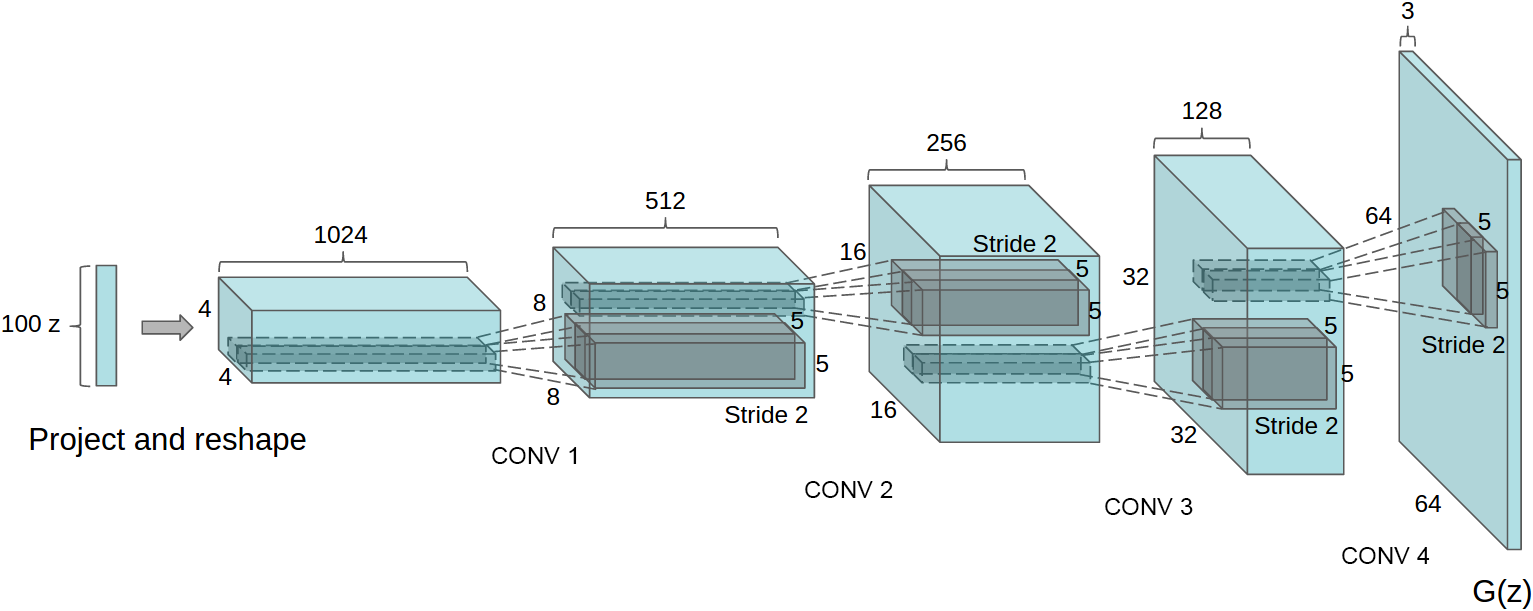
\includegraphics[width=\textwidth]{images/dcgan-architecture}
    \caption{DCGAN-Architektur des Generators von
    \cite{radford2016unsupervised}. Als Eingabe dient ein 100-dimensionaler
    Vektor, dessen Elemente zufällig gewählt werden. Dieser wird dann in den
    ersten Schichten umgeformt und durch vier Convolutional-Layer auf die Form
    3$\times$64$\times$64 gebracht. Die Strides geben dabei den
    Vergrößerungsfaktor pro Convolution-Schicht an, während die Anzahl der
    Filter den Farbkanälen entsprechen.}
  \end{figure}

  \section{Wasserstein GAN}
  Anders als andere GAN-Varianten verwendet das Wasserstein-GAN (WGAN) die
  Was\-ser\-stein-Distanz anstelle der JS- oder KL-Divergenz, um die Gewichte
  von generativen neuronalen Netzen zu optimieren. Da sich die Berechnung aller
  möglichen gemeinsamen Verteilungen $\gamma \sim \Pi(P_r, P_\theta)$ etwas schwierig
  gestaltet, formt \cite{arjovsky2017wasserstein} die Definition unter
  Berücksichtigung der Kontorovich-Rubinstein-Dualität um, sodass
  \[
    W(P_r, P_\theta) = \sup_{\|f\|_L \leq 1} \mathbb{E}_{x \sim P_r}\left[f(x)\right] - \mathbb{E}_{x \sim P_\theta}\left[f(x)\right]
  \]

  gilt, wobei das Supremum über alle 1-Lipschitz-Funktionen $f : X \to
  \mathbb{R}$ ist. Zusätzlich wird ein kleiner Trick angewendet, um das Problem
  weiter zu vereinfachen, indem K-Lipschitz-kontinuierliche Funktionen verwendet
  werden.
  \[
    K \cdot W(P_r, P_\theta) = \sup_{\|f\|_L \leq K} \mathbb{E}_{x \sim P_r}\left[f(x)\right] - \mathbb{E}_{x \sim P_\theta}\left[f(x)\right]
  \]

  Nehmen wir nun an, dass die Abbildung $f \in \left\{f_w\right\}_{w \in W}$
  parametrisiert durch $w$ existiert, wobei $W$ die Menge aller möglichen
  Parameter darstellt, so können die Parameter $w$ und damit die Abbildung $f_w$
  von einem neuronalen Netz erlernt werden, um so die Wasserstein-Distanz
  effizient abzuschätzen. Hier bildet der Wasserstein-Abstand also gleichzeitig
  die Loss-Funktion des Kritisierer mit
  \[
    W(P_r, P_\theta) = \max_{w \in W} \mathbb{E}_{x \sim P_r}\left[f_w(x)\right]
    - \mathbb{E}_{z \sim P_r(z)}\left[f_w(g_\theta(z))\right].
  \]

  Trotzdem darf nicht vergessen werden, dass dies nur gültig ist, falls die
  Funktion 1-Lipschitz-kontinuierlich ist. Um dies zu erzwingen, werden die
  Werte der aktualisierten Gewichte des Kritisierer zwischen $\left[-c; c\right]$
  gehalten. Dabei muss laut \cite{arjovsky2017wasserstein} $c$ relativ klein
  sein.

  \begin{algorithm}
    \SetAlgoLined
    \KwIn{Lernrate $\alpha$, Clipping-Parameter $c$, Batch-Größe
    $m$, Anzahl von Kritisierer-Iterationen $n_{critic}$.}
    \KwResult{Trainieren der Kritisierer-Parameter
    $w$ und Generator-Parameter $\theta$.}
    \caption{Wasserstein GAN nach \cite{arjovsky2017wasserstein}. Standardwerte
    für die Eingabeparameter sind $\alpha = 5\cdot10^{-5}, c = 0.01, m = 64$
    und $n_{critic} = 5$.}
    \label{alg:wgan}
    \BlankLine

    \While{$\theta$ \textnormal{ist nicht konvergiert}}{
      \For{$t = 0, ..., n_{critic}$}{
        Erzeuge Batch $\left\{x_i \;\lvert\; 1 \leq i \leq m\right\} \sim
        \mathbb{P}_r$ aus realen Daten\;
        Erzeuge Batch $\left\{z_i \;\lvert\; 1 \leq i \leq m\right\} \sim
        \mathbb{P}_z$ aus latenten Vektoren\;
        \BlankLine
        $g_w \leftarrow
        \nabla_w \left[ \frac{1}{m}\sum_{i=1}^{m} f_w(x_i) -
        \frac{1}{m}\sum_{i=1}^{m} f_w(g_\theta(z_i)\right]$\;
        \BlankLine
        $w \leftarrow w + \alpha \cdot \mathrm{RMSProp}(w,
        g_w)$\;
        $w \leftarrow \mathrm{clip}(w, -c, c)$\;
      }
      \BlankLine
      Erzeuge Batch $\left\{z_i \;\lvert\; 1 \leq i \leq m\right\} \sim
      \mathbb{P}_z$ aus latenten Vektoren\;
      $g_\theta \leftarrow -\nabla_\theta \left[\frac{1}{m} \sum_{i=1}^{m}
      f_w(g_\theta(z_i))\right]$\;
      $\theta \leftarrow \theta - \alpha \cdot \mathrm{RMSProp}(\theta,
      g_\theta)$\;
    }
  \end{algorithm}

  Zusätzlich ist bei Wasserstein-GANs von einem Kritisierer (Critic) anstatt
  eines Diskriminators die Rede. Der Grund dafür ist, dass ein Diskriminator
  zwischen \textit{fake} und \textit{real} unterscheidet, mehr nicht. Der
  Kritisierer führt diese Unterteilung der Eingabeparameter nicht durch, sondern
  bewertet bzw. kritisiert diese viel mehr. Mathematisch ausgedrückt sprechen
  wir hierbei von einer linearen Ausgabe in $\mathbb{R}$ im Falle des
  Kritisierers, während der Diskriminator eine binäre Ausgabe erzeugt.  Zu
  Beginn von Algorithmus \ref{alg:wgan} werden die Parameter $w$ für den
  Kritisierer und $\theta$ für den Generator initialisiert. Anschließend werden
  $m$ Datenpunkte bzw. ein Batch aus dem reellen Datensatz (Verteilung
  $\mathbb{P}_r$) gezogen. Dies muss nicht unbedingt zufällig sein. Auch werden
  $m$ zufällige Vektoren erzeugt, die als Eingabe für den Generator dienen,
  welcher wiederum Fake-Daten erzeugt. Dabei bilden die Ausgaben des Generators
  eine eigene Verteilung $\mathbb{P}_\theta$.  Ziel des Generators ist es nun,
  die Distanz zwischen den beiden Verteilungen $\mathbb{P}_r, \mathbb{P}_\theta$
  zu minimieren, um möglichst realitätsnahe Ausgaben erzeugen zu können. Als
  nächstes werden die Gradienten $g_w$ für Parameter $w$ mithilfe von
  Gradient-Descent, dargestellt als $\nabla_w$, berechnet. Hierfür wird die
  Wasserstein-Distanz als Loss-Funktion verwendet.  Der nächste Schritt besteht
  daraus, die Parameter $w$ des Kritisierer-Netzwerks mithilfe des
  RMSprop-Algorithmus zu aktualisieren und die aktualisierten Gewichte so gering
  wie möglich zu halten, um die K-Lipschitz-Kontinuität zu gewährleisten. Dies
  wird mithilfe der Funktion $\mathrm{clip}$ umgesetzt, welche die
  Parameterwerte in einem bestimmten Intervall $\left[-c; c\right]$ festsetzt.
  Die bis hier erläuterten Schritte werden $n_{critic}$-mal durchgeführt, sodass
  das Kritisierer-Netzwerk immer öfter trainiert wird, als der Generator. Dieser
  wird nun optimiert, indem wieder $m$ Vektoren zufällig erzeugt und als Eingabe
  für das Generator-Netzwerk verwendet werden. Der Generator erzeugt damit $m$
  zufällige Ausgaben, die wiederum als Eingaben in das Kritisierer-Netzwerk
  gegeben werden. Aus den Ausgaben wird dann der Mittelwert gebildet und zum
  Bestimmen der Gradienten von den Generator-Parametern $\theta$ verwendet.

  Im direkten Vergleich zu dem originalen GAN \cite{goodfellow2014generative}
  werden einige Änderungen in der Architektur vorgenommen. Während in dem
  originalen Anstatz fast nach jeder Schicht eine Batch-Normalization
  vorgenommen wird, können diese bei WGANs entfallen. Standard-GANs würden
  hierbei kaum interpretierbare Resultate erzeugen, WGANs hingegen produzieren
  trotzdem gute Ergebnisse, wie Experimente von \cite{arjovsky2017wasserstein}
  zeigen (siehe Abbildung \ref{fig:wgan-gan-no-batchnorm}). Das Wasserstein-GAN
  hat zusätzlich noch einige nützliche Eigenschaften. So wird unter anderem
  durch Annäherung des Wasserstein-Abstandes zwischen Generator- und
  Ausgangsdistribution das Problem des Mode-Collapse gelöst.  Durch den
  Wasserstein-Abstand wird der Abstand zwischen den Verteilung wesentlich besser
  minimiert (im Falle des Generator-Modells) als bei der KL- oder JS-Divergenz.
  Die Ausgabe eines Kritisierers stellt damit eine Bewertung der Eingabe dar,
  anstatt diese einer Klasse zuzuweisen und besitzt deshalb mehr Aussagekraft.

  \begin{figure}
    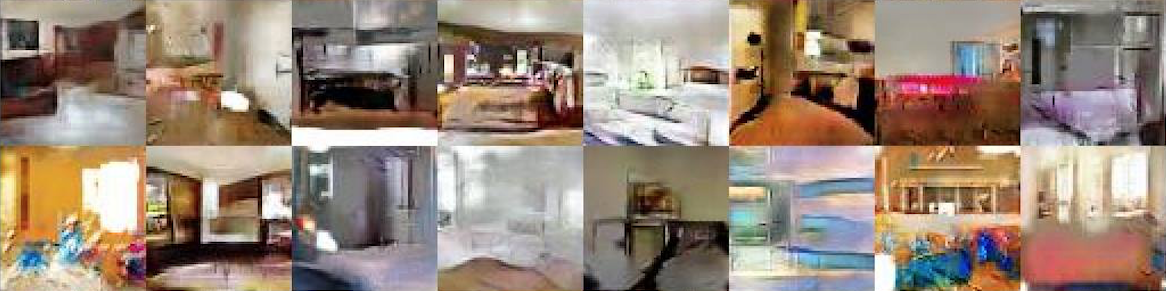
\includegraphics[width=0.5\textwidth]{images/image-022.png}
    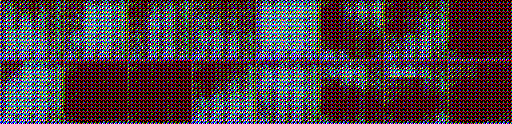
\includegraphics[width=0.5\textwidth]{images/image-024.png}
    \caption{Vergleich von WGAN und Standard-GAN \cite{arjovsky2017wasserstein}.
      Links sind Ausgaben vom WGAN-Algorithmus zu sehen während rechts Ausgaben
      eines Standard-GANs dargestellt sind. In beiden Generator-Modellen wurden
      Batch-Normalization-Layer entfernt. Klar zu erkennen ist, dass WGAN immer
      noch interpretierbare Ergebnisse liefert während bei Standard-GANs Probleme
      erkennbar sind.}
    \label{fig:wgan-gan-no-batchnorm}
  \end{figure}

  \section{Wasserstein-GAN mit Gradient-Penalty}
  Ein großes Problem von Wasserstein-GANs ist das Clippen der Gewichte in ein
  fest definiertes Intervall, um die 1-Lipschitzstetigkeit zu erfüllen. Das dies
  keine elegante Lösung ist, liegt auf der Hand. In \cite{gulrajani2017improved}
  wurde speziell dieses Problem genauer untersucht und es wurde festgestellt,
  dass das Beschneiden der Gewichte den Kritisierer dazu verleitet, nur extrem
  einfache Funktionen zu erlernen, wie der Vergleich in Abbildung
  \ref{fig:problems-of-weight-clipping} zeigt. 

  Um das Problem des Weight-Clippings anzugehen, stellt
  \cite{gulrajani2017improved} eine alternative Lösung vor, die auf anderem Wege
  die 1-Lipschitzstetigkeit in WGANs sicherstellen soll. Hierbei soll
  Gradient-Penalty helfen und wird als
  \[
    (\|\nabla_{\hat{x}} D(\hat{x})\| - 1)^2
  \]
  berechnet, wobei $\hat{x} =  x \epsilon + \tilde{x}(1 - \epsilon)$ eine
  zufällige Gewichtung zwischen realen ($x$) und generierten Daten ($\tilde{x}$)
  darstellt. Das $\epsilon$ wird dabei zufällig aus $\left[0, 1\right]$ gewählt.
  Daraus resultierend gestaltet sich die neue Loss-Funktion des Kritisierers wie
  folgt.
  \[
    L = \mathbb{E}_{\tilde{x} \sim \mathbb{P}_g}\left[D(\tilde{x})\right] -
        \mathbb{E}_{x \sim \mathbb{P}_r}\left[D(x)\right] +
        \lambda \cdot \mathbb{E}_{\hat{x} \sim \mathbb{P}_{\hat{x}}}\left[(\|\nabla_{\hat{x}} D(\hat{x})\| - 1)^2\right]
  \]
  Der Kritisierer ist durch diese Änderung nun wesentlich besser dazu in der
  Lage, komplexere Verteilungen zu erlernen.

  \begin{algorithm}
    \caption{WGAN mit Gradient-Penalty \cite{gulrajani2017improved}.}
    \KwIn{Gradient-Penalty-Koeffizient $\lambda$, Anzahl von Kritisierer-Iterationen
    $n_{critic}$, Batch-Größe $m$, Adam-Hyperparameter $\alpha, \beta_1,
    \beta_2$.}
    \KwResult{Trainieren der Kritisierer-Parameter $w$ und Generator-Parameter
    $\theta$.}
    \BlankLine
    \While{$\theta$ \textnormal{ist nicht konvergiert}}{
      \For{$t = 1, ..., n_{critic}$}{
        \For{$i = 1, ..., m$}{
          Wähle reale Probe $x \sim \mathbb{P}_r$, latenten Vektor $\vec{z} \sim
          \mathbb{P}_z$, zufällige Zahl $\epsilon \in \left[0, 1\right]$\;
          $\tilde{x} \leftarrow G_\theta(\vec{z})$\;
          $\hat{x} \leftarrow x\epsilon + \tilde{x}(1 - \epsilon)$\;
          $L_i = D_w(\tilde{x}) - D_w(x) + \lambda(\|\nabla_{\hat{x}}
          D_w(\hat{x})\| - 1)^2$\;
        }
        \BlankLine
        $w \leftarrow \mathrm{Adam}(\nabla_w \frac{1}{m} \sum_{i=1}^m L_i, w,
        \alpha, \beta_1, \beta_2)$\;
      }
      \BlankLine
      Wähle einen Batch aus latenten Vektoren $\{\vec{z}_i\}_{i=1}^m \sim
      \mathbb{P}_z$\;
      $\theta \leftarrow \mathrm{Adam}(\nabla_{\theta} \frac{1}{m} \sum_{i=1}^m
      - D_w(G_\theta(\vec{z}_i)), \theta, \alpha, \beta_1, \beta_2)$\;
    }
  \end{algorithm}

  \begin{figure}
    \centering
    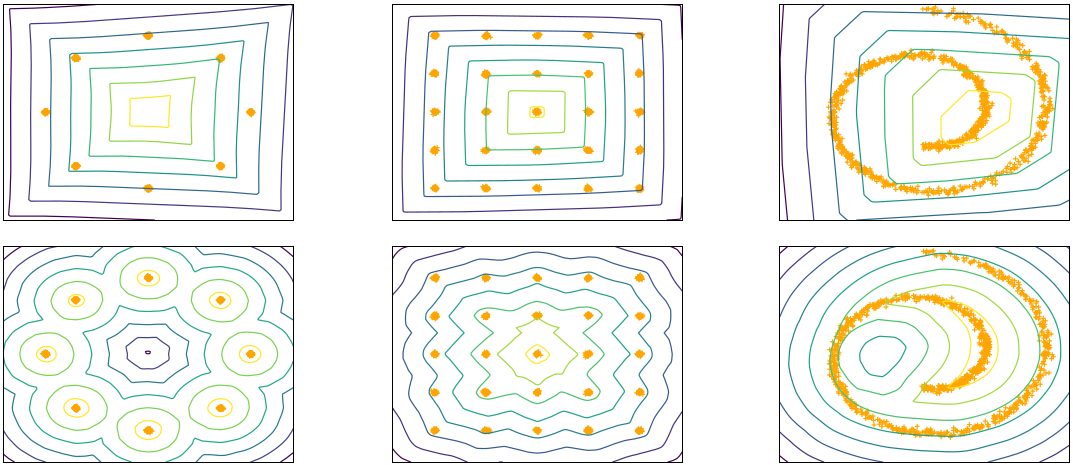
\includegraphics[width=\textwidth]{images/problems_of_weight_clipping}
    \caption{Vergleich zwischen Weight-Clipping (oben) und Gradient-Penalty
    (unten). Man erkennt deutlich, dass die Separierung der Ausgangsverteilung,
    dargestellt durch orangene Punkte, durch Weight-Clipping in sehr
    vereinfachte Funktionen resultiert. Gradient-Penalty lässt hingegen
    komplexere Strukturen von Verteilungen zu \cite{gulrajani2017improved}.}
    \label{fig:problems-of-weight-clipping}
  \end{figure}

  \chapter{Erstellen eines Datensatzes}\label{chapter:dataset}
  \section{Rahmenbedingungen}
  \section{Verwendung von GANs}
  \section{Durchführung von Experimenten mit unterschiedlichen GANs}
  \section{Analyse der Ergebnisse aus den Experimenten}

  \chapter{Bewegungserkennung}\label{chapter:motion-detection}
  \section{Erkennung von Bewegungsarten}
  \section{Erkennung von Anomalien}
  \section{Erkennung von Eigenschaften}
  \section{Vorhersage von Bewegungen}
  \section{Architektur einer mobilen Anwendung}

  \chapter{Fazit und Ausblick}

  \printbibliography
\end{document}
